\section{Model transformations}
\label{sec:ch7_ModelTransformations}
This section explains the model transformations required for modelling, analysing, and mapping the \gls{ibc} system using \gls{sadf}. 
The model transformations are required to obtain the implementation-aware \gls{ibc} graph from the \gls{ibc} graph for the given design parameters, as illustrated in Fig.~\ref{fig:ch7_ibc_overview}.  
Our model transformations consist of maximising parallelism, creating a pipe, replicating pipes to implement pipelining, introducing camera-awareness, introducing workload-awareness, modelling inter-frame dependencies, and re-timing of actor execution times.
For each workload scenario, we assume that the sensing and processing task is modelled as an \gls{sdfg} $\SDFG_{\taskS}$, the control computation task is modelled as an \gls{sdfg} $\SDFG_{\taskC}$, and the actuation task is modelled as an \gls{sdfg} $\SDFG_{\taskA}$.
The graphs $\SDFG_{\taskS},\ \SDFG_{\taskC},$ and $\SDFG_{\taskA}$ should have identifiable source and sink actors $a_{src,i}$ and $a_{snk,i},\ i\in\{\taskS,\taskC,\taskA\}$.
A source is an actor without any incoming edges and a sink is an actor without any outgoing edges.
We moreover enforce that $\repetitionVector(a_{src,i})=%1$ and $
\repetitionVector(a_{snk,i})=1$. 
Having identifiable source and sink actors with repetition-vector entries equal one ensures well-formedness for our model transformations.
Note that an \gls{sdfg} with a single actor satisfies the assumptions. The source and sink actors should be identical across all workload \glspl{sdfg} in an application \gls{ibc} \gls{sadf}.

To maximize opportunities to speed up the computations in the control loop, we want to maximize parallelism in graphs $\SDFG_{\taskS},\ \SDFG_{\taskC},$ and $\SDFG_{\taskA}$. Automatically extracting task- and data parallelism in computations is challenging. So, in general, it is up to the designer to maximize parallelism in the three mentioned graphs. But given an \gls{sdfg} of a workload scenario, it is possible to maximize data parallelism by transforming the \gls{sdfg} to a \gls{hsdfg}~\cite{lee1987synchronous,sriram2018embedded}. Essentially, this transformation replicates actors with a repetition-vector entry greater than one into multiple actors (as many as the repetition-vector entry of the actor for the \gls{sdfg}) with each a repetition-vector entry one in the \gls{hsdfg}. A platform-aware mapping such as implemented in the SDF3 tool~\cite{stuijk2006sdf} then clusters actors of the \gls{hsdfg} per processor in the given platform allocation for maximising throughput.
A disadvantage of this approach, however, is the scalability of the mapping and performance analysis that depends on the number of actors.

Another option is to replicate the parallelisable actors as many times as meaningful given the platform allocation. That is, we transform an \gls{sdfg} $\SDFG$ via a transformation
$\transformParallel(\SDFG,\replicationVector)$ that preserves the number and timing of firings in a single iteration of the original graph $\SDFG$ in the transformed graph, where $\replicationVector$ is the replication vector with size equal to the number of actors in $\SDFG$ and where each element $\replicationVector(a)$ represents the number of times an actor $a$ needs to be replicated.
A straightforward replication vector can then be defined using the repetition vector $\repetitionVector$ and the maximum number of processing cores allocated for parallel execution of tasks per pipe $\numCoresParallel$, as $\replicationVector(a)=min(\repetitionVector(a),\numCoresParallel),\ a\in \Actors$. Often, this transformation is relatively straightforward, but a definition that works in general is not obvious. The challenge when replicating actors is to accurately model the transformations of channels, production and consumption rates, and initial tokens such that the functional and timing behaviour of the original graph is preserved.
Fig.~\ref{fig:ch7_transformParallel} gives some example transformations, including Gantt charts that illustrate that actor firings and their timing are preserved. We leave a generic definition (and the proof that such a transformation exists in general and preserves functionality and timing) as future work. Note that the \gls{sdfg}-to-\gls{hsdfg} transformation of~\cite{lee1987synchronous,sriram2018embedded} is an instance of $\transformParallel$ when the replication vector is chosen equal to the repetition vector.

 \begin{figure}[ht]
        \centering
        \begin{subfigure}[b]{0.4\textwidth}
            \centering
            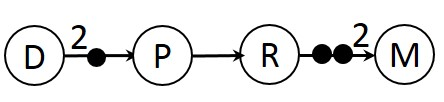
\includegraphics[width=.8\textwidth]{images/G1.jpg} 
             \caption{{$\SDFG_1$ }}
             \label{fig:ch7_G1}
        \end{subfigure}
        \hspace*{1cm}
        \begin{subfigure}[b]{0.4\textwidth}  
            \centering 
            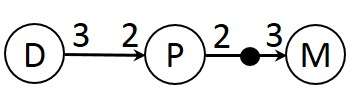
\includegraphics[width=0.7\textwidth]{images/G2.jpg}
             \caption{{$\SDFG_2$ }}
             \label{fig:ch7_G2}
        \end{subfigure}
        \vskip\baselineskip
        \begin{subfigure}[b]{0.4\textwidth}   
            \centering 
            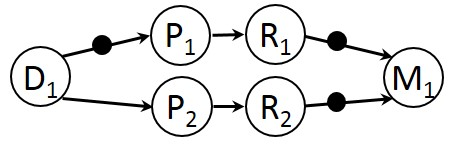
\includegraphics[width=.8\textwidth]{images/G1repA.jpg}
            \caption{{$\transformParallel(\SDFG_1,[1\ 2\ 2\ 1])$}}
            \label{fig:ch7_G1repA}
        \end{subfigure}
        \hspace*{1cm}
        \begin{subfigure}[b]{0.4\textwidth}   
            \centering 
            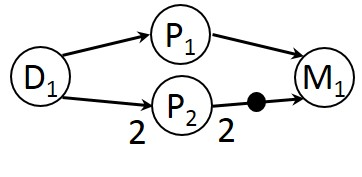
\includegraphics[width=0.7\textwidth]{images/G2repA.jpg}
            \caption{{$\transformParallel(\SDFG_2,[1\ 2\ 1])$ }}
            \label{fig:ch7_G2repA}
        \end{subfigure}
        \vskip\baselineskip
        \begin{subfigure}[b]{0.4\textwidth}   
            \centering 
            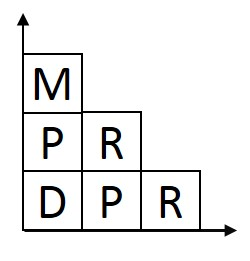
\includegraphics[scale=0.4]{images/GanttG1.jpg}
            \caption{{Gantt chart for~\ref{fig:ch7_G1} and~\ref{fig:ch7_G1repA}
            }}
        \end{subfigure}
        \hspace*{1cm}
        \begin{subfigure}[b]{0.4\textwidth}   
            \centering 
            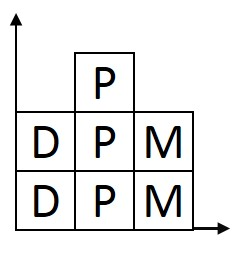
\includegraphics[scale=0.4]{images/GanttG2.jpg}
            \caption{{Gantt chart for~\ref{fig:ch7_G2} and~\ref{fig:ch7_G2repA}
            }}
        \end{subfigure}
        \caption{{Examples of the replicate actors $\transformParallel$ transformation. The Gantt charts cover one iteration of the corresponding graph and assume actor execution times to be 1. Subscripts resulting from $\transformParallel$ transformations are omitted for brevity.}} 
        \label{fig:ch7_transformParallel}
        \vspace{-1em}
\end{figure}

For the remainder, assume that $\SDFG_{\taskS}$, $\SDFG_{\taskC}$, and $\SDFG_{\taskA}$ are the graphs obtained after maximizing parallelism. The \textbf{Create pipe} $\transformSequential(\SDFG_{\taskS},\SDFG_{\taskC},\SDFG_{\taskA})$ transformation creates a model for a single pipe by adding a delay actor and channels between the sinks and sources of $\SDFG_{\taskS}$ and $\SDFG_{\taskC}$, $\SDFG_{\taskC}$ and $\SDFG_{\taskA}$, $\SDFG_{\taskA}$ and delay, and delay and $\SDFG_{\taskS}$. 
The execution time of the delay actor is set to zero, and one initial token is added to the channel between the delay actor and the source of $\SDFG_{\taskS}$ to enforce sequential implementation of the pipe (see Fig.~\ref{fig:ch7_transformations}).
The latency of the resulting \gls{sdfg} can be configured by an appropriate choice of the execution time of the delay actor (which can be set using the re-timing transformation given in Def.\ \ref{def:transformFixTiming}).
The model transformation results in an \gls{sdfg} whose latency is equal to the inverse of the throughput.

\begin{definition}
{\textbf{(Create pipe $\transformSequential(\SDFG_{\taskS},\SDFG_{\taskC},\SDFG_{\taskA})$)}}~\label{def:transformSequential}
Transformation $\transformSequential(\SDFG_{\taskS},\SDFG_{\taskC},\SDFG_{\taskA})$ creates a single pipe and sequentialises the graph execution (by restricting pipelining). $\transformSequential(\SDFG_{\taskS},\SDFG_{\taskC},\SDFG_{\taskA})= (\Actors^{\prime},\ \Channels^{\prime},\ \actorET^{\prime},\ \ratesSDFG_p^{\prime},\ \ratesSDFG_c^{\prime},\ \initialTokens^{\prime})$ with
\begin{align}
\Actors^{\prime}&=\Actors_{\taskS}\ \cup\ \Actors_{\taskC}\ \cup\ \Actors_{\taskA}\ \cup\ \{\text{delay}\},\nonumber\\ \Channels^{\prime}&=\Channels_{\taskS}\ \cup\ \Channels_{\taskC}\ \cup\ \Channels_{\taskA} \nonumber %\\ &
\ \ \cup\ \{c_1=(a_{snk,\taskS},a_{src,\taskC}),\ c_2=(a_{snk,\taskC},a_{src,\taskA}),\nonumber\\ &\ \hspace*{2cm} c_3=(a_{snk,\taskA},\text{delay}),\ c_4=(\text{delay},a_{src,\taskS})\},\nonumber\\
\actorET^{\prime}&=\actorET_{\taskS}\ \cup\ \actorET_{\taskC}\ \cup\ \actorET_{\taskA}\ \cup\ \{(\text{delay},0))\},\nonumber\\
\ratesSDFG_p^{\prime}&=\ratesSDFG_{p_{\taskS}}\ \cup\ \ratesSDFG_{p_{\taskC}}\ \cup\ \ratesSDFG_{p_{\taskA}}\ \cup\ \{(c_1,1),(c_2,1),(c_3,1),(c_4,1)\},\nonumber\\
\ratesSDFG_c^{\prime}&=\ratesSDFG_{c_{\taskS}}\ \cup\ \ratesSDFG_{c_{\taskC}}\ \cup\ \ratesSDFG_{c_{\taskA}}\ \cup\ \{(c_1,1),(c_2,1),(c_3,1),(c_4,1)\},\nonumber\\
\initialTokens^{\prime}&=\initialTokens_{\taskS}\ \cup\ \initialTokens_{\taskC}\ \cup\ \initialTokens_{\taskA}\ \cup\ \{(c_1,0),(c_2,0),(c_3,0),(c_4,1)\}. \nonumber
\end{align}
\end{definition}

The $\transformSequential$ transformation is essential to compute sensor-to-actuator delay $\tau$ for our implementations. To compute $\tau_i$ for a workload scenario $s_i$: i) compute $\transformSequential(\transformParallel(\SDFG_{{\taskS}_i},\parallelisationVector_{{\taskS}_i}),\transformParallel(\SDFG_{{\taskC}_i},\parallelisationVector_{{\taskC}_i}),\transformParallel(\SDFG_{{\taskA}_i},\parallelisationVector_{{\taskA}_i}))$; ii) map the transformed graph to the given platform allocation to obtain the binding-aware graph $\bindingAwareSDFG{i}$; and iii) compute the latency of $\bindingAwareSDFG{i}$. This latency value is equal to $\tau_i$. 

The replicate-pipe transformation is an intermediate step in the model transformation, where we replicate the entire pipe to enable pipelining (see Fig.~\ref{fig:ch7_transformations}, $\transformReplicate(g_1,2)$).
Since each actor can be mapped to only one processing core, implementing pipelining on multiple processing cores is challenging without replication of a single pipe.
 $\transformReplicate(\SDFG,d)$ facilitate the modelling for a pipelined implementation with $d$ pipes. 
 Recall that a pipe is created from $\SDFG_{\taskS}$, $\SDFG_{\taskC}$ and $\SDFG_{\taskA}$ (see Definition~\ref{def:transformSequential}). These subgraphs in a single pipe are all replicated $d$ times by the replicate-pipe transformation. The $\transformReplicate$ transformation does not use the specifics of the graph it is applied to. It generically replicates the entire \gls{sdfg} the specified number of times.

\begin{definition}
{\textbf{(Replicate pipe $\transformReplicate(\SDFG,d)$)}}
Let $\SDFG = (\Actors,\ \Channels,\ \actorET,\ \ratesSDFG_p,\ \ratesSDFG_c,\ \initialTokens)$ be an \gls{sdfg}. 
Transformation $\transformReplicate(\SDFG,d)$ replicates the \gls{sdfg} $d$ times resulting in $\transformReplicate(\SDFG,d)= (\Actors^{\prime},\ \Channels^{\prime},\ \actorET^{\prime},\ \ratesSDFG_p^{\prime},\ \ratesSDFG_c^{\prime},\ \initialTokens^{\prime})$
with
\begin{align}
 \Actors^{\prime}&=\bigcup_{a\in\Actors}\ \{a_j\ |\ 1\le j\le d\}\footnotemark, \nonumber\\ \actorET^{\prime}&=\{(a_j,e(a))\ |\ a\in\Actors, \ 1\le j\le d\}, \nonumber\\
 \Channels^{\prime}&=\bigcup_{c\in\Channels}\ \{c_j\ |\ 1\le j\le d\}, \nonumber\\
 \initialTokens^{\prime}&=\{(c_j,\initialTokens(c))\ |\ c\in\Channels, \ 1\le j\le d\}, \nonumber\\
\ratesSDFG_p^{\prime}&= \{(c_j,\ratesSDFG_p(c))\ |\ c\in\Channels, \ 1\le j\le d\},\nonumber\\ 
\ratesSDFG_c^{\prime}&=\{(c_j,\ratesSDFG_c(c))\ |\ c\in\Channels, \ 1\le j\le d\}. \nonumber
\end{align}
\footnotetext{This union replicates every actor in the original graph $d$ times. For every actor $a$ in $\Actors$, we create $a_{1},\dots,\ a_d$ actors in the new graph.}
\end{definition}

\begin{figure}[t]
    \centering
    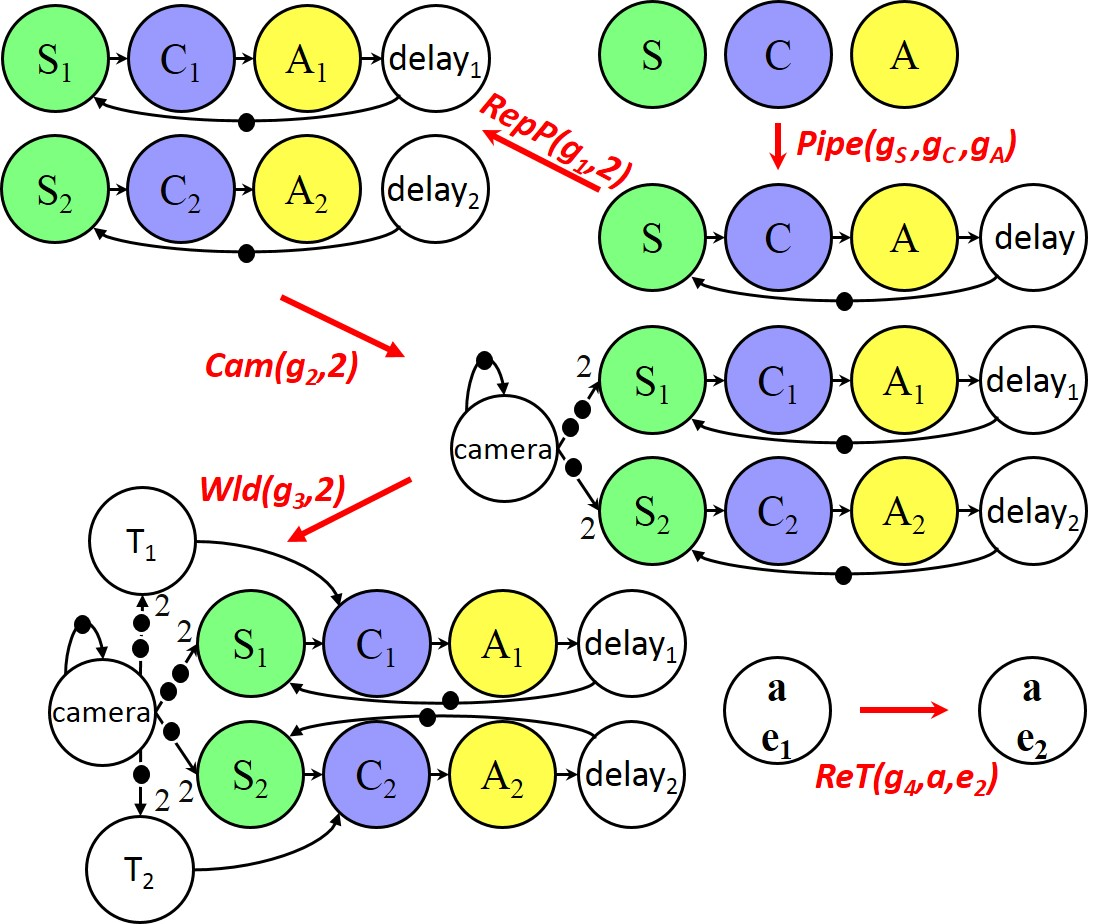
\includegraphics[width=0.7\textwidth]{images/transformations.jpg}
    \caption{Illustration of model transformations.}
    \label{fig:ch7_transformations}
\end{figure}

 The three following transformations - adding camera-awareness, workload-awareness and inter-frame dependencies - assume that the replicate-pipe transformation has been performed with replication factor $d$ on a single pipe created with transformation $\transformSequential$, optionally preceded by replicate-actor transformations (which do not affect these transformations).
 
 
The \textbf{Camera-awareness} transformation is an intermediate step in our model transformations. 
It adds a camera actor with execution time equal to the inverse of the given camera frame rate (the frame arrival period $\fh$), a self-edge with an initial token to model the frame arrival, and channels from the camera actor to the $d$ replicated source actors ${a_{src,{\taskS}}}_j$ with the channel consumption rate equal to the number of replications $d$ (see Fig.~\ref{fig:ch7_transformations}, $\transformCamera(g_2,2)$). The number of initial tokens in these channels are set to enforce an ordering of the pipes in the pipelined implementation.
\begin{definition}
{\textbf{(Camera-awareness $\transformCamera(\SDFG,d)$)}}
% ~\label{def:transformCamera}
Let $\SDFG = (\Actors,\ \Channels,\ \actorET,\ \ratesSDFG_p,\ \ratesSDFG_c,\ \initialTokens)$ be the \gls{sdfg} $\transformReplicate(\transformSequential(\SDFG_{\taskS},\SDFG_{\taskC},\SDFG_{\taskA}),$ $d)$. 
Transformation $\transformCamera(\SDFG,d)= (\Actors^{\prime},\ \Channels^{\prime},\ \actorET^{\prime},\ \ratesSDFG_p^{\prime},\ \ratesSDFG_c^{\prime},\ \initialTokens^{\prime})$ enforces a camera frame rate, with
\begin{align}
\Actors^{\prime}&=\Actors\ \cup\ \{\text{camera}\},\ \actorET^{\prime}=\actorET\ \cup\ \{(\text{camera},\fh)\}, \nonumber\\
\Channels^{\prime}&=\Channels\ \cup\ \{(\text{camera})^2\}\ \cup\nonumber\\ &\hspace*{10mm}\{c_j=(\text{camera},a_{src,{{\taskS}_j}})\ |\ 1\le j\le d\}, \nonumber\\
\ratesSDFG_p^{\prime}&=\ratesSDFG_p\ \cup\ \{((\text{camera})^2,1)\}\ \cup\ \{(c_j,1)\ |\ 1\le j\le d\},\nonumber\\
\ratesSDFG_c^{\prime}&=\ratesSDFG_c\ \cup\ \{((\text{camera})^2,1)\}\ \cup\ \{(c_j,d)\ |\ 1\le j\le d\},\nonumber\\
\initialTokens^{\prime}&=\initialTokens\cup\{((\text{camera})^2,1)\}\cup\{(c_j,d-j+1)\ |\ 1\le j\le d\}.\nonumber
\end{align}

\end{definition}

The \textbf{Workload-awareness} transformation is a step in the model transformations performed on graph $\transformCamera(\transformReplicate(\transformSequential(\SDFG_{\taskS},\SDFG_{\taskC},\SDFG_{\taskA}),d),d)$.
Due to image-workload variations, the sensing task's runtime execution times are varying. 
Also, for the \gls{spade} implementation, the system scenarios may abstract multiple workload scenarios with varying execution times for the sensing task.
However, the \gls{spade} controller design requires a constant sensor-to-actuator delay per system scenario for the implementation.
The $\transformWorkload$ transformation enforces a constant sensor-to-actuator delay for our implementation.
The $\transformWorkload$ transformation adds actors $T_j$ with an incoming channel from the camera actor and an outgoing channel to the (replicated) source actor ${a_{src,{\taskC}}}_j$ of the computation \gls{sdfg} $\SDFG_{\taskC}$.
The consumption rate and initial tokens for the channels from camera actor to $T_j$ are the same as for the channel from camera actor to source actors in the $\transformCamera$ transformation, again to enforce ordering in the pipelined execution (see Fig.~\ref{fig:ch7_transformations}, $\transformWorkload(g_3,2)$).
The $T_j$ actors create a path in parallel to the $\SDFG_{\taskS}$ graph instances. By setting the execution time of these added $T_j$ actors to an appropriately large value, a constant sensor-to-actuator delay can be enforced. The $\transformWorkload$ transformation sets the execution time to 0. The execution-time value can be updated when needed in the \gls{spade} flow by the re-timing transformation introduced below.

\begin{definition}
{\textbf{(Workload-awareness $\transformWorkload(\SDFG,d)$)}}
% ~\label{def:transformWorkload}
Let $\SDFG = (\Actors,\ \Channels,\ \actorET,\ \ratesSDFG_p,\ \ratesSDFG_c,\ \initialTokens)$ be the \gls{sdfg} $\transformCamera(\transformReplicate($ $\transformSequential(\SDFG_{\taskS},\SDFG_{\taskC},\SDFG_{\taskA}),d),d)$. 
Transformation $\transformWorkload(\SDFG)= (\Actors^{\prime},\ \Channels^{\prime},$ $ \actorET^{\prime},\ \ratesSDFG_p^{\prime},\ \ratesSDFG_c^{\prime},\ \initialTokens^{\prime})$, with
\begin{align}
\Actors^{\prime}&=\Actors\ \cup\ \{T_j\ |\ 1\le j\le d\},\nonumber\\ \actorET^{\prime}&=\actorET\ \cup\ \{(T_j,0)\ |\ 1\le j\le d\}, \nonumber\\
\Channels^{\prime}&=\Channels\ \cup\ \{cT_j=(\text{camera},T_j)\ |\ 1\le j\le d\}\  \cup \nonumber\\
&\hspace*{10mm} \{TC_j=(T_j,{a_{src,{\taskC}}}_j)\ |\ 1\le j\le d\}, \nonumber\\
\ratesSDFG_p^{\prime}&=\ratesSDFG_p\ \cup\ \{(cT_j,1)\ |\ 1\le j\le d\}\ \cup \nonumber\\
&\hspace*{10mm} 
\{(TC_j,1)\ |\ 1\le j\le d\},\nonumber\\
\ratesSDFG_c^{\prime}&=\ratesSDFG_c\ \cup\ \{(cT_j,d)\ |\ 1\le j\le d\}\ \cup \nonumber\\
&\hspace*{10mm} 
\{(TC_j,1)\ |\ 1\le j\le d\},\nonumber\\
\initialTokens^{\prime}&=\initialTokens\ \cup\ \{(cT_j,d-j+1)\ |\ 1\le j\le d\}\ \cup \nonumber\\
&\hspace*{10mm} 
\{(TC_j,0)\ |\ 1\le j\le d\}.\nonumber
\end{align}
\end{definition}

The \textbf{inter-frame-dependency} transformation adds channels to enforce the dependencies for actor firings between two consecutive pipes. 
E.g., an actor $b_j$ that executes in the $k$-th pipe might depend on the completion of execution of an actor $a_i$ that executes in the $(k-1)$-th pipe.
This transformation is optionally done after $\transformCamera$ (and has no further effect on the definition of the earlier transformations).
An example for this transformation is illustrated in Fig.~\ref{fig:ch7_transformationIFD}.
Ideally, our model transformations ensure that the inverse throughput of the implementation-aware graph is equal to the execution time of the camera actor. E.g. if $\actorET($camera$)=\fh$, then the throughput of the implementation-aware graph is equal to (or limited by) the camera frame rate $\frac{1}{\fh}$.
Now, the $\transformIFD$ transformation allows the throughput to be limited also by the inter-frame dependencies.
The inverse throughput of the implementation-aware graph will then be equal to the maximum of $\actorET($camera$)$ and the inter-frame dependence time $\fd$ (as explained later in Section~\ref{sec:ch7_IFD}).

%\vspace{5mm}
\begin{definition}
{\textbf{(Inter-frame dependency $\transformIFD(\SDFG,a,b,d)$)}}
% ~\label{def:transformInterFrameDependency}
Let $\SDFG = (\Actors,\ \Channels,\ \actorET,\ \ratesSDFG_p,\ \ratesSDFG_c,\ \initialTokens)$ be the \gls{sdfg} $\transformCamera(\transformReplicate($ $\transformSequential(\SDFG_{\taskS},\SDFG_{\taskC},\SDFG_{\taskA}),d),d)$. 
Transformation $\transformIFD(\SDFG,a,b,d)= (\Actors,\ \Channels^{\prime},\ \actorET,\ $ $ \ratesSDFG_p^{\prime},\ \ratesSDFG_c^{\prime},\ \initialTokens^{\prime})$ adds inter-frame dependencies between actors $a_i$ and $b_j$, for $a_i,b_j\in\Actors$, with 
\begin{align}
 \Channels^{\prime}&= \Channels\ \cup\ \{c_d=(a_d,b_1)\}\ \cup\ \{c_j=(a_{j},b_{j+1}) \ |\ 1\le j< d\}, \nonumber\\
\ratesSDFG_p^{\prime}&=\ratesSDFG_p\ \cup\ \{(c_d,\repetitionVector(b_1))\}\ \cup\ \{(c_j,\repetitionVector(b_{j+1})) \ |\ 1\le j< d\},\nonumber\\ 
\ratesSDFG_c^{\prime}&=\ratesSDFG_c\ \cup\ \{(c_d,\repetitionVector(a_d))\}\ \cup\ \{(c_j,\repetitionVector(a_{j})) \ |\ 1\le j< d\},\nonumber\\ 
\initialTokens^{\prime}&=\initialTokens\ \cup\ \{(c_d,\repetitionVector(a_d)))\}\ \cup\ \{(c_j,0) \ |\ 1\le j< d\}.\nonumber
\end{align}
\end{definition}

\begin{figure}[ht]
    \centering
    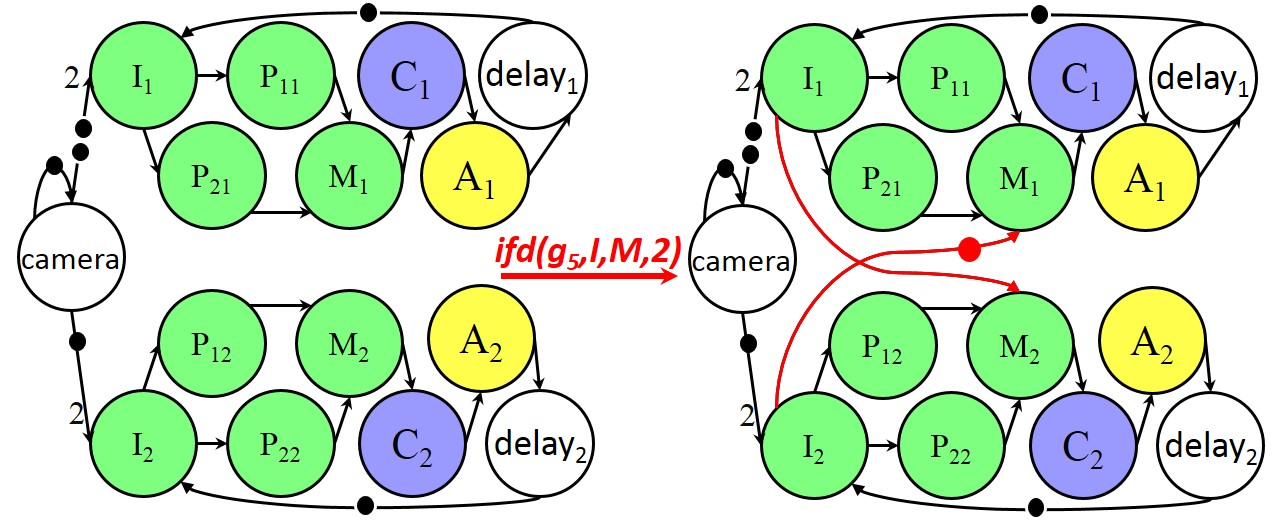
\includegraphics[width=0.8\textwidth]{images/transformIFD.jpg}
    \caption{Illustration of inter-frame dependencies between the actors I and M. The channels added by $\transformIFD(g_5,I,M,2)$ are shown in red.}
    \label{fig:ch7_transformationIFD}
\end{figure}

During \gls{spade} analysis, the $\tau$ and $h$ values are updated based on our implementation choices. The \textbf{re-timing} transformation helps to update the execution time of the actors (camera, delay, and T) in our models when required (see Fig.~\ref{fig:ch7_transformations}, $\transformFixTiming(g_4,a,e_2)$). 

\begin{definition}
{\textbf{(Re-timing $\transformFixTiming(\SDFG,a,t)$)}}~\label{def:transformFixTiming}
Let $\SDFG = (\Actors,\ \Channels,\ \actorET,\ \ratesSDFG_p,\ \ratesSDFG_c,\ \initialTokens)$ be an SDFG. 
Transformation $\transformFixTiming(\SDFG,a,t)= (\Actors,\ \Channels,\ \actorET^{\prime},\ \ratesSDFG_p,\ \ratesSDFG_c,\ \initialTokens)$ updates the execution time of actor $a\in\Actors$ to $t\in  \R_{\geq 0}$, with 
\begin{equation}
\actorET^{\prime}=\actorET\ \setminus\ \{(a,\actorET(a))\} \cup\ \{(a,t)\}.  \nonumber
\end{equation}
\end{definition}